% Options for packages loaded elsewhere
% Options for packages loaded elsewhere
\PassOptionsToPackage{unicode}{hyperref}
\PassOptionsToPackage{hyphens}{url}
%
\documentclass[
  ignorenonframetext,
]{beamer}
\newif\ifbibliography
\usepackage{pgfpages}
\setbeamertemplate{caption}[numbered]
\setbeamertemplate{caption label separator}{: }
\setbeamercolor{caption name}{fg=normal text.fg}
\beamertemplatenavigationsymbolsempty
% remove section numbering
\setbeamertemplate{part page}{
  \centering
  \begin{beamercolorbox}[sep=16pt,center]{part title}
    \usebeamerfont{part title}\insertpart\par
  \end{beamercolorbox}
}
\setbeamertemplate{section page}{
  \centering
  \begin{beamercolorbox}[sep=12pt,center]{section title}
    \usebeamerfont{section title}\insertsection\par
  \end{beamercolorbox}
}
\setbeamertemplate{subsection page}{
  \centering
  \begin{beamercolorbox}[sep=8pt,center]{subsection title}
    \usebeamerfont{subsection title}\insertsubsection\par
  \end{beamercolorbox}
}
% Prevent slide breaks in the middle of a paragraph
\widowpenalties 1 10000
\raggedbottom
\AtBeginPart{
  \frame{\partpage}
}
\AtBeginSection{
  \ifbibliography
  \else
    \frame{\sectionpage}
  \fi
}
\AtBeginSubsection{
  \frame{\subsectionpage}
}
\usepackage{iftex}
\ifPDFTeX
  \usepackage[T1]{fontenc}
  \usepackage[utf8]{inputenc}
  \usepackage{textcomp} % provide euro and other symbols
\else % if luatex or xetex
  \usepackage{unicode-math} % this also loads fontspec
  \defaultfontfeatures{Scale=MatchLowercase}
  \defaultfontfeatures[\rmfamily]{Ligatures=TeX,Scale=1}
\fi
\usepackage{lmodern}

\usetheme[]{metropolis}
\ifPDFTeX\else
  % xetex/luatex font selection
\fi
% Use upquote if available, for straight quotes in verbatim environments
\IfFileExists{upquote.sty}{\usepackage{upquote}}{}
\IfFileExists{microtype.sty}{% use microtype if available
  \usepackage[]{microtype}
  \UseMicrotypeSet[protrusion]{basicmath} % disable protrusion for tt fonts
}{}
\makeatletter
\@ifundefined{KOMAClassName}{% if non-KOMA class
  \IfFileExists{parskip.sty}{%
    \usepackage{parskip}
  }{% else
    \setlength{\parindent}{0pt}
    \setlength{\parskip}{6pt plus 2pt minus 1pt}}
}{% if KOMA class
  \KOMAoptions{parskip=half}}
\makeatother


\usepackage{longtable,booktabs,array}
\usepackage{calc} % for calculating minipage widths
\usepackage{caption}
% Make caption package work with longtable
\makeatletter
\def\fnum@table{\tablename~\thetable}
\makeatother
\usepackage{graphicx}
\makeatletter
\newsavebox\pandoc@box
\newcommand*\pandocbounded[1]{% scales image to fit in text height/width
  \sbox\pandoc@box{#1}%
  \Gscale@div\@tempa{\textheight}{\dimexpr\ht\pandoc@box+\dp\pandoc@box\relax}%
  \Gscale@div\@tempb{\linewidth}{\wd\pandoc@box}%
  \ifdim\@tempb\p@<\@tempa\p@\let\@tempa\@tempb\fi% select the smaller of both
  \ifdim\@tempa\p@<\p@\scalebox{\@tempa}{\usebox\pandoc@box}%
  \else\usebox{\pandoc@box}%
  \fi%
}
% Set default figure placement to htbp
\def\fps@figure{htbp}
\makeatother

\ifLuaTeX
  \usepackage{luacolor}
  \usepackage[soul]{lua-ul}
\else
  \usepackage{soul}
  \makeatletter
  \let\HL\hl
  \renewcommand\hl{% fix for beamer highlighting
    \let\set@color\beamerorig@set@color
    \let\reset@color\beamerorig@reset@color
    \HL}
  \makeatother
\fi




\setlength{\emergencystretch}{3em} % prevent overfull lines

\providecommand{\tightlist}{%
  \setlength{\itemsep}{0pt}\setlength{\parskip}{0pt}}



 


\setbeamerfont{title}{size=\large} \usepackage{hyperref} \setbeamertemplate{footline}[frame number]
\makeatletter
\@ifpackageloaded{caption}{}{\usepackage{caption}}
\AtBeginDocument{%
\ifdefined\contentsname
  \renewcommand*\contentsname{Table of contents}
\else
  \newcommand\contentsname{Table of contents}
\fi
\ifdefined\listfigurename
  \renewcommand*\listfigurename{List of Figures}
\else
  \newcommand\listfigurename{List of Figures}
\fi
\ifdefined\listtablename
  \renewcommand*\listtablename{List of Tables}
\else
  \newcommand\listtablename{List of Tables}
\fi
\ifdefined\figurename
  \renewcommand*\figurename{Figure}
\else
  \newcommand\figurename{Figure}
\fi
\ifdefined\tablename
  \renewcommand*\tablename{Table}
\else
  \newcommand\tablename{Table}
\fi
}
\@ifpackageloaded{float}{}{\usepackage{float}}
\floatstyle{ruled}
\@ifundefined{c@chapter}{\newfloat{codelisting}{h}{lop}}{\newfloat{codelisting}{h}{lop}[chapter]}
\floatname{codelisting}{Listing}
\newcommand*\listoflistings{\listof{codelisting}{List of Listings}}
\makeatother
\makeatletter
\makeatother
\makeatletter
\@ifpackageloaded{caption}{}{\usepackage{caption}}
\@ifpackageloaded{subcaption}{}{\usepackage{subcaption}}
\makeatother

\usepackage{bookmark}
\IfFileExists{xurl.sty}{\usepackage{xurl}}{} % add URL line breaks if available
\urlstyle{same}
\hypersetup{
  pdfauthor={Giorgio Arcara},
  hidelinks,
  pdfcreator={LaTeX via pandoc}}


\author{Giorgio Arcara}
\date{}

\begin{document}


\begin{frame}
% TITLE SLIDES
\title{Metodi Statistici per la Neuropsicologia Forense\\ \vspace{1em} \emph{4c. Affidabilità (formule)}}
\author{Giorgio Arcara,\\ Università di Padova \\ IRCCS San Camillo, Venezia}

\titlegraphic{

\vspace*{7cm}

\includegraphics[scale=0.15]{Figures/LogoSanCamilloIRCCS_Unipd_alpha.png}
\hfill 
\includegraphics[scale=0.15]{Figures/CC_license_3_0.png}
}
\maketitle
\end{frame}

\begin{frame}{Affidabilità}
\phantomsection\label{affidabilituxe0}
\begin{center}
  \textbf{Tipi di affidabilità}
\end{center}
\vspace{2em}

\begin{itemize}
\tightlist
\item
  Affidabilità test-retest
\item
  Affidabilità inter-rater
\item
  Consistenza interna
\end{itemize}

\vspace{2em}

Esistono diverse classificazioni di affidabilità. Questa è
principalmente basata su Urbina, 2004, Essentials of Psychological
Testing.
\end{frame}

\section{Affidabilità test-retest}\label{affidabilituxe0-test-retest}

\begin{frame}{Affidabilità test-retest}
\phantomsection\label{affidabilituxe0-test-retest-1}
\textbf{Affidabilità test-retest}: è un indice che rappresenta la
consistenza nel tempo di due misurazioni assumendo che non è avvenuto
nessun cambiamento sistematico.

La formula standard e più diffusa quella della correlazione di Pearson
(vedi anche l'Appendice di queste slides):

\[
r = \frac{\sum (x_i - \bar{x})(y_i - \bar{y})}
{\sqrt{\sum (x_i - \bar{x})^2 \sum (y_i - \bar{y})^2}}
\]

\[
\small
\begin{aligned}
r & = \text{correlation coefficient} \\
x_i & = \text{values of the x-variable in a sample} \\
\bar{x} & = \text{mean of the values of the x-variable} \\
y_i & = \text{values of the y-variable in a sample} \\
\bar{y} & = \text{mean of the values of the y-variable}
\end{aligned}
\]
\end{frame}

\begin{frame}{Affidabilità test-retest}
\phantomsection\label{affidabilituxe0-test-retest-2}
Il più grande problema dell'affidabilità test retest è che essa non
cattura eventuali effetti sistematici di differenza tra i punteggi. Il
valore infatti ci dice quanto due valori sono correlati o consistenti,
ma non se sono più o meno gli stessi.

Immaginiamo un caso in cui ad ogni osservazione si aggiunga una quantità
fissa \(k\). Conseguirà che anche la media sarà aumentata di \(k\):

\[
r = \frac{\sum (x_i - \bar{x})(y_i + k - (\bar{y} + k))}
{\sqrt{\sum (x_i - \bar{x})^2 \sum (y_i + k - (\bar{y} + k))^2}}
\] Segue da semplice algebra che le ``k'' si cancellano e quindi si
ritorna alla formula iniziale: un aumento sistematico non cambia il
valore della correlazione (vedi anche slides su Correlazione
nell'Appendice concetti base di statistica)
\end{frame}

\begin{frame}{Affidabilità test-retest}
\phantomsection\label{affidabilituxe0-test-retest-3}
Nei test cognitivi l'effetto sistematico più comune è riconducibile
all'effetto pratica, l'etichetta utilizzata per indigare quei
cambiamenti (spesso sistematici) che si osservano nella somministrazione
del test e che sono associati ad una migliore performance.

Attenzione dunque all'utilizzo e all'interpretazione dei valori di
test-retest relaibility che sono spesso (nei compiti cogntivi) solo
parziali per indicare la stabilità di una performance.

Sarebbero infatti da accompagnare da analisi (es. t-tests) che
permattano di vedere se c'è una differenza sistematica tra prima e
seconda valutazione.
\end{frame}

\begin{frame}{Affidabilità test-retest}
\phantomsection\label{affidabilituxe0-test-retest-4}
\begin{center}
  \textbf{Considerazioni su affidabilità test-retest}
\end{center}

Spesso l'affidabilità test-retest viene (erroneamente) considerata utile
solo nel caso in cui avvengano misurazioni ripetute.

Dobbiamo invece immaginare una valutazione come una fotografia di una
scena statica. La affidabilità test-retest stima quanto è precisa la
vostra macchina fotografica.

In un test ad elevata affidabilità, non ci aspettiamo tante possibili
variazioni, invece in un test con bassa affidabilità ci aspettiamo molte
variazioni.

La nostra fotografia sarà una stima ``puntuale'', ma potrebbe essere
lontana da quella che consideriamo il punteggio vero (che ricordiamo è
un'entità teorica).
\end{frame}

\begin{frame}{Affidabilità test-retest}
\phantomsection\label{affidabilituxe0-test-retest-5}
\begin{center}
  \textbf{Considerazioni su affidabilità test-retest}
\end{center}

Nella slide successiva si mostra questo concetto, ipotizzando delle
singole misurazioni m\(_a\) ed m\(_b\) in due test (uno a bassa
affidabilità test-retest e uno ad alta affidabilità test-retest).

Per ogni test verrà fatta una sola valutazione e non c'è interesse nella
rivalutazione nel tempo. Nel test con alta affidabilità test-retest,
avremo un punteggio osservato che è meno dipendente dalla specifica
istanza di misurazione.
\end{frame}

\begin{frame}{Affidabilità test-retest}
\phantomsection\label{affidabilituxe0-test-retest-6}
\begin{columns}
  \begin{column}{0.5\textwidth}
    \begin{figure}
    \includegraphics[scale=0.25]{Figures/affidabilità_test_retest.png}
    \end{figure}
  \end{column}
  \begin{column}{0.5\textwidth}
    Test bassa affidabilità test-retest
    
    \vspace{6em}
    Test alta affidabilità test-retest
  \end{column}
\end{columns}
\end{frame}

\begin{frame}{Affidabilità test-retest}
\phantomsection\label{affidabilituxe0-test-retest-7}
Perché viene usato il coefficiente di correlazione di Pearson (\(r\)) se
non è adeguato? \vspace{2em}

Probabilmente per semplice convenzione e per semplicità (il coefficiente
r di pearson può esprimere facilmente la varianza condivisa tra le
variabili, semplicemente calcolando \(r^2\)).

Non è completamente sbagliato e può fornire un quadro abbastanza
completo se accompagnato da t-tests (per indagare differenze
sistematiche).
\end{frame}

\section{Affidabilità inter-rater}\label{affidabilituxe0-inter-rater}

\begin{frame}{Affidabilità inter-rater}
\phantomsection\label{affidabilituxe0-inter-rater-1}
\small

\textbf{Affidabilità inter-rater}: è un'indice che rappresenta la
coerenza dei punteggi di piùrater.

La formula più utilizzata per l'affidabilità inter-rater è
l'\textbf{Intra Class Correlation (ICC)}.

A differenza della correlazione (che può essere usata solo per 2
variabili), l'ICC invece può essere usata per \(k\) variabili (dove
\(k\) è il numero di raters).

Esistono diverse formule di Intraclass correlation, che sostanzialmente
rispondono a diverse domande e che assumono una diversa relazione tra
gruppi e osservazioni (nel nostro caso raters e pazienti osservati). Le
formule più recenti per intraclass correlation si basano su
scomposizione di varianza fatta tramite ANOVA o tramite mixed effect
models (utile da sapere ma non approfondiamo).

\href{https://en.wikipedia.org/wiki/Intraclass_correlation}{\ul{https://en.wikipedia.org/wiki/Intraclass\_correlation}}
\end{frame}

\begin{frame}{Affidabilità inter-rater}
\phantomsection\label{affidabilituxe0-inter-rater-2}
\small

La versione di ICC più utilizzata per calcolare l'affidabilità
inter-rater è la \textbf{ICC(2,1) agreement}.

Nel contesto di test con questa versione di ICC si assume che
\underline{più rater vedano la stessa prestazione dello stesso soggetto}
e fornisce una stima che tiene conto dell'agreement in termini assoluti
(se il punteggio è lo stesso, non se il punteggio è correlato).

\[
ICC(2,1) = \frac{(MSB - MSE)}
{(MSB + (n_j - 1)MSE + \frac{n_j(MSJ - MSE)}{n_c})}
\]

\[
\small
\begin{aligned}
MSB & = \text{variance between subjects} \\
MSJ & = \text{variance between judges (raters)} \\
MSE & = \text{variance of interaction judges by subjects} \\
n_c & = \text{number of judges (raters)} \\
n_j & = \text{number of cases (observations)}
\end{aligned}
\]
\end{frame}

\begin{frame}{Affidabilità inter-rater}
\phantomsection\label{affidabilituxe0-inter-rater-3}
\begin{columns}
  \begin{column}{0.5\textwidth}
    \begin{figure}
    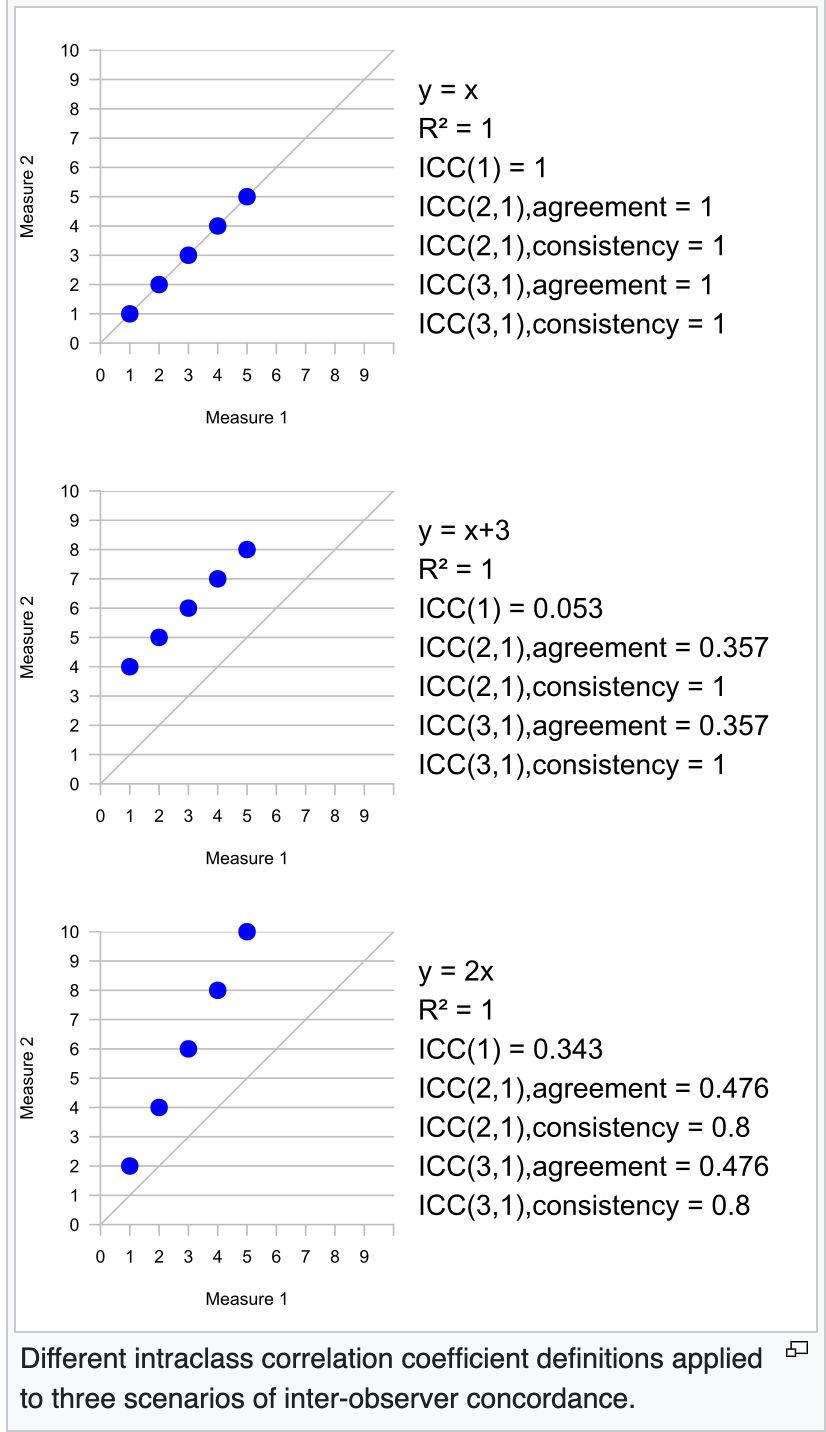
\includegraphics[scale=0.2]{Figures/wiki_ICC.png}
    \end{figure}
    \footnote{Da pagina Wikipedia Intraclass Correlation}
  \end{column}
  \begin{column}{0.5\textwidth}
    La figura mostra come diverse relazioni sono catturate da diversi coefficienti.
    
    Nota che $R^2$ è il coefficiente di correlazione $r$ elevato al quadrato, ma è anche usato nelle regressioni (in breve altre analisi statistiche dove si indaga la relazione tra variabili usando equazione del tipo $y = bx + e$).
  \end{column}
\end{columns}
\end{frame}

\begin{frame}{Affidabilità inter-rater}
\phantomsection\label{affidabilituxe0-inter-rater-4}
\begin{center}
  \textbf{Alcune considerazioni su ICC}
\end{center}

\textbf{Perché non è usata ICC anche per test-retest visto che tiene
conto anche di differenze sistematiche?}

Probabilmente più per prassi e convenzione. In letteratura è possibile
trovare alcuni studi che la utilizzano anche per test-retest. In caso di
effetto pratica sarebbe infatti più adeguata.
\end{frame}

\section{Consistenza interna}\label{consistenza-interna}

\begin{frame}{Consistenza interna}
\phantomsection\label{consistenza-interna-1}
\textbf{Consistenza interna}: rappresenta la consistenza tra gli item di
un test.

Un approccio tradizionale per calcolare la consistenza di item di un
test, è quella di dividere in due il test e indagare misure di
somiglianza (es. correlazione) tra i punteggi delle due metà nei vari
partecipanti. \textbf{Questo metodo è detto split-half reliability (o
affidabilità split-half)}.

Il grosso limite di questo approccio è che il risultato dipende da come
dividiamo a metà il test (potremmo sovrastimare o sottostimare).

Da un punto di vista concettuale le misure di consistenza interna vanno
ad indagare invece quale sarebbe la correlazione usando tutte le
possibili divisioni split-half.
\end{frame}

\begin{frame}{Consistenza interna}
\phantomsection\label{consistenza-interna-2}
\begin{center}
  \textbf{Formula di Kuder-Richardson (K-R 20)}
\end{center}

È una formula che viene usata quando gli item sono dicotomici (0/1)

\[
r_k-R20 = (\frac{n}{n-1})\frac{s_t^2 - \sum{pq}}{s_t^2}
\]

\[
\small
\begin{aligned}
n & = \text{numero di items nel test} \\
s_t^2 & = \text{varianza del punteggio totale nel test} \\
\sum{pq} & = \text{somma del prodotto $p$ x $q$ in ogni item del test} \\
p & = \text{proporzione delle persone che passano l’item (o risposta 1)} \\
q & = \text{proporzione delle persone che non passano l’item (o risposta 0)}
\end{aligned}
\]
\end{frame}

\begin{frame}{Consistenza interna}
\phantomsection\label{consistenza-interna-3}
\begin{center}
  \textbf{Cronbach's alpha}
\end{center}

È una generalizzazione della formula KR-20, nel caso di items non
dicotomici

\[
alpha = (\frac{n}{n-1})\frac{s_t^2 - \sum{s_i^2}}{s_t^2}
\]

\[
\small
\begin{aligned}
n & = \text{numero di items nel test} \\
s_t^2 & = \text{varianza del punteggio totale nel test} \\
s_i^2 & = \text{varianza di ogni item al test} \\
\end{aligned}
\]
\end{frame}

\begin{frame}{Consistenza interna}
\phantomsection\label{consistenza-interna-4}
\begin{center}
  \textbf{Altri metodi per consistenza interna}
\end{center}

Anche se i metodi KR-20 e alpha sono i più comuni essi hanno dei limiti
intrinseci (Es. Assumono unidimensionalità).

In alcuni quindi da preferire altri metodi. Esempio: se i punteggi degli
item non sono normali meglio il metodo \textbf{GLB (Greatest Lower
Bound)}.

In caso di multidimensionalità puà essere meglio usare il metodo
\textbf{omega (\(\omega\))}.

Nota che GLB e omega sono legati ad analisi fattoriali (vedi slides su
validità) e sono computazionalmente più complessi.
\end{frame}

\begin{frame}{Consistenza interna}
\phantomsection\label{consistenza-interna-5}
\begin{center}
  \textbf{Item selection}
\end{center}

\small

Un concetto associato a KR-20, Cronbach's alpha, e altre misure di
consistenza interna è quello dell'item selection e cioè quella procedura
nella creazione di un test di identificazione degli item da mantenere
nel test finale.

Alcune misure sono specifiche per items (un po' come I loadings
nell'analisi fattoriale).

Esempi che vengono dall'alpha di Cronbach:

\begin{itemize}
\item
  \textbf{r-drop}: indica la correlazione tra il test, e il test tolto
  quell'item (si ha dunque un valore r-drop per item)
\item
  \textbf{r-cor}: indica la correlazione tra l'item e il test totale
  controllando per overlap con altri item e per affidabilità globale.
\end{itemize}
\end{frame}

\begin{frame}{Affidabilità ed errore}
\phantomsection\label{affidabilituxe0-ed-errore}
\begin{center}
  \textbf{Interpretare l'affidabilità a livello del test}
\end{center}

\small

Ogni sorgente di affidabilità può essere usata per stimare l'errore di
misura del test.

Il coefficiente di affidabilità (indipendente dalla formula) può infatti
essere intrepretato come la percentuale di variabili riconducibile al
punteggio vero, trasformando semplicemente il coefficiente in
percentuale. Questo segue la definizione che viene fatta a priori di
cosa è l'affidabilità.

Ad esempio:

Una correlatione test-retest 0.8, vuol dire che 80\% di variabilità
test-retest è riconducibile alla variabilità del punteggio vero.

Una consistenza interna di 0.9, vuol dire che 90\% di variabilità nella
consistenza interna pè riconducibile alla variabilità del punteggio
vero, etc.
\end{frame}

\begin{frame}{Affidabilità ed errore}
\phantomsection\label{affidabilituxe0-ed-errore-1}
\begin{center}
  \textbf{Interpretare l'affidabilità a livello del test}
\end{center}

L'errore associato ad ogni sorgente di affidabilità è pertanto
calcolabile come:

\[
Errore = (1-C_a)*100
\] Dove \(C_a\) è il coefficiente di affidabilità in questione (es.
Affidabilità test retest, affidabilità inter rater, etc).
\end{frame}

\begin{frame}{Affidabilità ed errore}
\phantomsection\label{affidabilituxe0-ed-errore-2}
\begin{center}
  \textbf{Combinare diversi tipi di errore}
\end{center}

Calcolando diverse sorgenti di errore è possibile sommarle (assumendo la
loro indipendenza) per ottenere un errore totale e calcolare quindi la
variabilità del punteggio che si presume sia riconducibile al punteggio
vero

Es. supponiamo di avere un test che ha le seguenti caratteristiche:

\begin{itemize}
\tightlist
\item
  Affidabilità test-retest = 0.85 (\(r\) di pearson)
\item
  Affidabilità inter-rater = 0.70 (\(ICC(2,1)\))
\item
  Consistenza interna = 0.95 (alpha di Cronbach)
\end{itemize}
\end{frame}

\begin{frame}{Affidabilità ed errore}
\phantomsection\label{affidabilituxe0-ed-errore-3}
\begin{center}
  \textbf{Combinare diversi tipi di errore}
\end{center}

Errore test-retest: \((1-0.85) * 100 = 15%
\)

Errore inter-rater: \((1-0.7) * 100 = 30%
\)

Errore consistenza interna: \((1-0.95) = 5%
\)

Errore totale: \(15 + 30 + 5 = 50%
\) \vspace{2em}

A livello di test il 48\% della varianza è riconducibile ad errore, e il
52\% (100 -- 48) della varianza è riconducibile al punteggio vero (è
anche l'affidabilità complessiva del test).
\end{frame}

\begin{frame}{Affidabilità ed errore}
\phantomsection\label{affidabilituxe0-ed-errore-4}
\begin{center}
  \textbf{Stimare il punteggio vero}
\end{center}

Le formule di affidabilità ci permettono inoltre di stimare il punteggio
vero

\[
T'=r_{xx}(X-M)+M
\] \[
\small
\begin{aligned}
T' & = \text{stima del punteggio vero} \\
r_{xx} & = \text{affidabilità complessiva (vedi slide precedente)} \\
X & = \text{punteggio osservato} \\
M & = \text{media del campione di riferimento} \\
\end{aligned}
\]
\end{frame}

\begin{frame}{Affidabilità ed errore}
\phantomsection\label{affidabilituxe0-ed-errore-5}
\begin{center}
  \textbf{Stimare il punteggio vero: alcune note}
\end{center}

\begin{enumerate}
[1)]
\tightlist
\item
  La stima del punteggio vero è spesso accompagnata anche dalla
  creazione di intervalli di confidenza attorno alla stima (riprenderemo
  questo quando parleremo di cut-offs, vedi anche Appendice)
\end{enumerate}
\end{frame}

\begin{frame}{Affidabilità ed errore}
\phantomsection\label{affidabilituxe0-ed-errore-6}
\begin{center}
  \textbf{Stimare il punteggio vero: alcune note}
\end{center}

\small

\begin{enumerate}
[1)]
\setcounter{enumi}{1}
\tightlist
\item
  Per stimare il punteggio vero entra due volte in gioco la media del
  campione di riferimento (denotata con M). Questo permette di tenere in
  consdierazione un fenomeno detto \textbf{regressione verso la media}:
  in ogni misura con errore è sempre più probabile che una misura
  successiva sia più vicina alla media del campione di riferimento.
  Questo perché, specie se l'errore dello strumento è grande, ogni
  deviazione della media ha probabilità di essere dovuta al caso.
\end{enumerate}

Correggere per la media ha però un grosso limite intrinseco: con che
media correggere? Ad esempio, se ho un paziente con TBI è corretto usare
(per M), la media del gruppo di sani con cui è stato sviluppato il test?
\end{frame}

\begin{frame}{Affidabilità ed errore}
\phantomsection\label{affidabilituxe0-ed-errore-7}
\begin{center}
  \textbf{Stimare il punteggio vero: alcune note}
\end{center}

Questo tipo di limiti rende complessa l'applicazione di formule per
stimare il punteggio vero. Vedremo in futuro comunque in utilizzi
clinici e pratici (es. cut-off, valori di cambiamento),
\textbf{\underline{quasi sempre non sono usati i punteggi veri ma i punteggi osservati}}.
\end{frame}

\begin{frame}{Affidabilità e varianza}
\phantomsection\label{affidabilituxe0-e-varianza}
\begin{center}
  \textbf{Come considerare i coefficienti di affidabilità}
\end{center}

Ogni coefficiente di affidabilità, in generale stimare la variabilità
riconducibile al punteggio vero, rispetto alla variabilità totale (cioè
quella che si rileva nei osservati), utilizzando diverse formule (es.
\(r\) di pearson, \(ICC(2,1)\), etc.).

L'idea generale può essere espressa da questa formula.

\[
r_{xx} = \frac{\sigma_{true}}{\sigma_{tot}}
\]
\end{frame}




\end{document}
